% -------------------------------------------------------------------
% - NAME:        poster.tex
% - AUTHOR:      Reto Stauffer
% - BASED ON:    Jakob Messners version of this theme
% - DATE:        2014-09-29
% -------------------------------------------------------------------
% - DESCRIPTION: This is a demo template for portrait beamer poster
%                in the UIBK design 2017.
% -------------------------------------------------------------------
\pdfminorversion=4 % Fixed a bug where rendered pdf's were not readable on windows/acroread
\documentclass[final]{beamer} 

\usepackage{natbib}
\usepackage{pdfpages}

\usepackage[orientation=portrait,size=a0,scale=1.30]{beamerposter}
\usetheme[ncols=2]{uibkposter}
%% ------------------------------------------------------------------
%% Use the two lines above for portrait posters
%% ------------------------------------------------------------------

%\usepackage[orientation=landscape,size=a0,scale=1.30]{beamerposter}
%\usetheme[ncols=3,orangetheme]{uibkposter}
%% ------------------------------------------------------------------
%% Use the two lines above for landscape posters
%% The option 'orangetheme' can be used to switch the theme.
%% Additional options allowed:
%% - orangetheme: uses alternative color theme
%% - boxskip=X: set length for vskip before each box. Allows to
%%   adjust spacing between boxes.
%% ------------------------------------------------------------------

\headerimage{1}
%% ------------------------------------------------------------------
%% The theme offers four different header images based on the
%% corporate design of the university of innsbruck. Currently
%% 1, 2, 3 and 4 is allowed as input to \headerimage{...}. Default
%% or fallback is '1'.
%% ------------------------------------------------------------------

%% ------------------------------------------------------------------
%% The official corporate colors of the university are predefined and
%% can be used for e.g., highlighting something. Simply use
%% \color{uibkorange} or \begin{color}{uibkorange} ... \end{color}
%% Defined colors are:
%% - uibkorange, uibkblue, uibkgray, uibkgraym
%% Please note that there are two faculty colors (see definition above)
%% - uibkcol, uibkcoll
%% The frametitle color can be easily adjusted e.g., to black with
%% \setbeamercolor{titlelike}{fg=black}
%% ------------------------------------------------------------------

%\setbeamercolor{verbcolor}{fg=uibkorange}
%% ------------------------------------------------------------------
%% Setting a highlight color for verbatim output such as from
%% the commands \pkg, \email, \file, \dataset 
%% ------------------------------------------------------------------

%% The title of your poster
\title{Testing the importance of explicit glacier dynamics for future glacier evolution in the Alps}

%% If the subtitle is not set or empty no subtitle will be shown
\subtitle{}

%% Author(s) of the poster
\author{Moritz Oberrauch (\textit{moritz.oberrauch@uibk.ac.at}), Fabien Maussion} 

%% Enable numbered captions (figures, tables)
\setbeamertemplate{caption}[numbered]

%% Begin document
\begin{document}

\begin{frame}[fragile]
\begin{columns}[t]

%% ------------------------------------------------------------------
%% This template contains content for both, the portrait version (two
%% columns) and the landscape version (three columns).
%% If \usepackage[orientation=portrait,...]{beamerposter} then the
%% center column is unused (only left and right column). In this
%% case simply remove the block:
%%     \if@beamerposter@portrait
%%         [...]
%%     \fi
%% If \usepackage[orientation=landscape]{beamerposter} the layout 
%% comes with three columns (left, center, right). In this case
%% remove the \if@beamerposter@portrait, \else and \fi condition but
%% keep the block:
%%     \begin{centercolumn}
%%         [...]
%%     \end{centercolumn}
%% ------------------------------------------------------------------

%% ------------------------------------------------------------------
%% begin left column for both, portrait and landscape
%% ------------------------------------------------------------------
\begin{leftcolumn}
   %% please leave one blank line here

   %% Introduction
   \begin{boxblock}{Volume-area scaling vs. shallow ice approximation}
      Even though the \textbf{Open Global Glacier Model (OGGM)} is a rather simple model (concerning the implemented physics), the \textbf{volume-area scaling (VAS) glacier model} originally used by \citet{Marzeion2012} is even more basic. While the OGGM implements shallow ice approximation to drive the model glacier, the VAS model relies solely on volume/area and volume/length scaling principles.
      \vspace{0.3cm}
      \textbf{What am I doing?!} Currently I'm implementing the original volume/area scaling model used by Ben (at least I'm trying to).
      \vspace{0.3cm}
      \textbf{Why am I doing it?!} More complex models generelly come with higher computational costs. While this may be necessary for certain detailed analysis, not all scientific questions call for such a high degree of accuracy. In addition, alpine glaciers will most likely not advance much in the coming decades. Hence, ice dynamics play a secondary role compared to ice melt.
      \vspace{0.3cm}
      \textbf{What do I want to achieve?!} In a nutshell: how far can I dumb the dynamic model down, while still producing reasonable results on a regional  scale. To do so I will:
      \begin{enumerate}
         \item implement glacier model(s) with different levels of complexity in the OGGM framework.
         \item investigate the strengths and weaknesses of the VAS model approach (sensitivity analysis).
         \item complete regional comittment runs for the alpine region (past and future).
      \end{enumerate}
   \end{boxblock}

   %% Mass balance
   \begin{boxblock}{Mass balance model}
      % The \textbf{mass balance model} is quite similar to the one used by the OGGM.
      The mass balance model implements a the \textbf{temperature index model}.
      \begin{align}
         B(t) = \left[\sum_{i=1}^{12}(P_i^\text{solid} - \mu^* \cdot \max(T_i^\text{teminus} - T_\text{melt}, 0))\right] - \beta^*
      \end{align}
      The annual specific surface mass balance $B(t)$ is computed as the difference of monthly solid precipitation fallen onto the glacier surface $P_i^\text{solid}$ (mass input) and monthly positive melting temperature at the glacier terminus $T_i^\text{teminus}$ (energy input), summed over a year. The temperature sensitivity parameter $\mu^*$ needs to be calibrated for every single glacier. Additionally, a mass balance bias $\beta^*$ can be added/subtracted.
      

      % It uses monthly temperature and precipitation data as input, which are scaled to the given glacier elevation. The main difference to the OGGM model is, that it computes a single (average) value of melting temperature and solid precipitation for the entire glacier.
      
   \end{boxblock}

   % Scaling
   \begin{boxblock}{The scaling model}
      The used scaling laws are quite basics:
      \begin{align}
         V(t) = c_A \cdot A(t)^\gamma, \qquad
         V(t) = c_L \cdot L(t)^q
      \end{align}
      where $c_A$, $c_L$ and $\gamma$, $q$ are scaling parameters.
      % where $c_A$ and $c_L$ are scaling constants and $\gamma$ and $q$ are scaling exponents for the area/volume and length/volume scaling, repecitvely.
      For each year $t$ the volume change $dV(t)$ is computed, given the specific mass balance $B(t)$ and the surface area $A(t)$. The resulting new volume $V(t+1)$ is used to compute the area change $dA$ and length change $dL$, scaled by the corresponding response time $\tau_A$ and $\tau_L$, resp. A change in glacier length $L(t+1)$ translates into a change in terminus elevation $z_\text{term}(t)$, which influences the specific mass balance $B(t+1)$.
      \begin{figure}
         \centering
         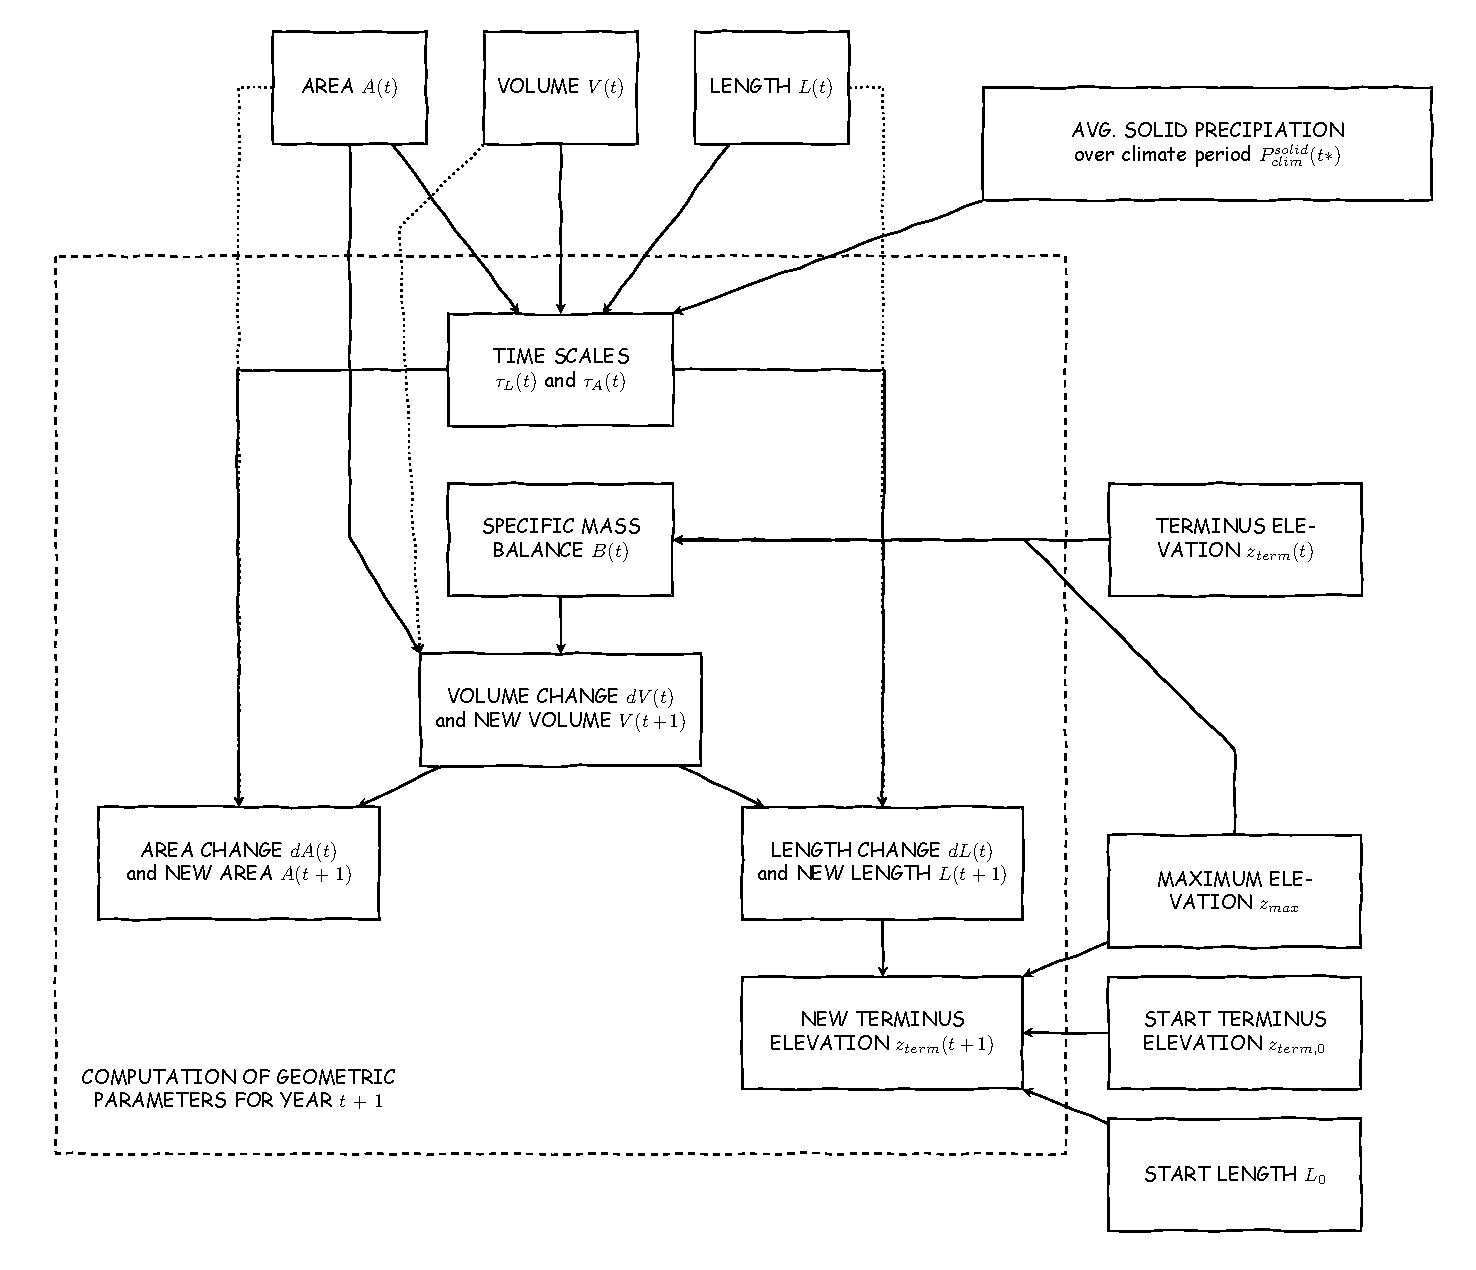
\includegraphics[width=1\textwidth]{../flowchart/scaling.pdf}
         \label{fig:flowchart}
      \end{figure}

   
   \end{boxblock}

\end{leftcolumn} %% end left column


%% ------------------------------------------------------------------
%% begin right column for both, portrait and landscape
%% ------------------------------------------------------------------
\begin{rightcolumn}
   %% please leave one blank line here

   % Comparison
   \begin{boxblock}{Comparing the model performance on a single glacier}
      Both models are initialized with the glacier outline of Hintereisferner in 2003 \citep{RGI}, without any spinup. The models run from 1802 to 2014 using the HistAlp climate data \citep{Auer2007} as input. Hence, the shown glacial evolution is a predominantly \textbf{qualitative result}, not comparable with the actual evolution of the Hintereisferener.
      \begin{figure}
         \centering
         \includegraphics[width=0.92\textwidth]{../plots/{RGI60-11.00897_volume}.png}
         \vspace*{1cm}
         \includegraphics[width=0.46\textwidth]{../plots/{RGI60-11.00897_length}.png}
         \hspace*{0.05\textwidth}
         \includegraphics[width=0.46\textwidth]{../plots/{RGI60-11.00897_area}.png}
         \label{fig:hef_timeseries}
      \end{figure}


   \end{boxblock}

   %% Commitment runs
   \begin{boxblock}{First small scale regional run - Rofental}
      Let's see if I produce something sensible here, until it has to be printed...
      \begin{figure}
         \centering
         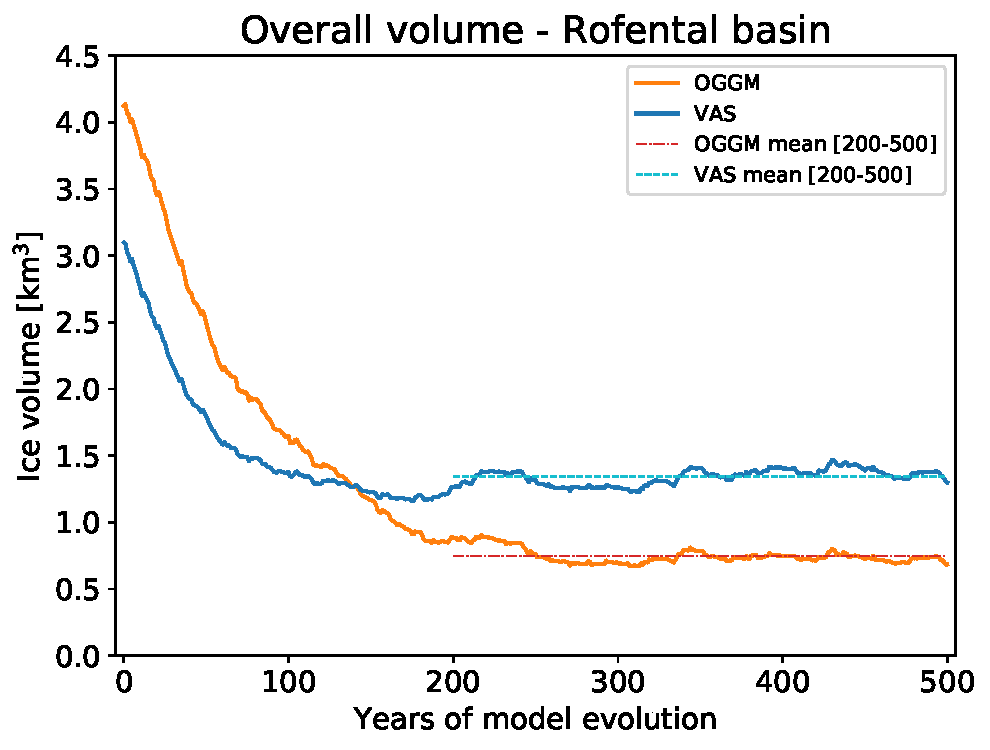
\includegraphics[width=0.92\textwidth,height=15cm]{../plots/rofental.png}
         \label{fig:rofenthal}
      \end{figure}
      
   \end{boxblock}

   %% What next?!
   \begin{boxblock}{What next?!}
      Given that this is just the first implementation step, the (qualitative) results are quite promising. However, some more work is required before deriving any conclusions. This includes the following tasks/questions:
      \begin{itemize}
         \item Does the length change have to be comparable?!
         \item Finding appropiate/sensible start values...
         \item Performance test against reference glaciers.
         \item Regional (alpine) runs
         \item Sensibility analysis
      \end{itemize}
      
   \end{boxblock}

   %% References
   \begin{footnotesize}

   \textbf{References:} \\
   \bibliographystyle{ametsoc}
   \bibliography{master}
   
   \vspace{0.3cm}
   \begin{minipage}[t]{0.75\textwidth}
      \textbf{Acknowledgements:} \\
      My thanks go to Ben Marzeion for clearifying some definitions and for supplying me with his original code base. Additional thanks go to my supervisor, Fabien Maussion.
   \end{minipage}
   \hfill
   \begin{minipage}[t]{0.12\textwidth}
      \begin{figure}
         \includegraphics[width=\textwidth]{license_ccby}
      \end{figure}
   \end{minipage}
   \end{footnotesize}
\end{rightcolumn}
%% end right column %%%%%%%%%%%%%%%%%%%%%%%%%%%%%%%%%%%%%%%%%%%%%%%%%%
%%%%%%%%%%%%%%%%%%%%%%%%%%%%%%%%%%%%%%%%%%%%%%%%%%%%%%%%%%%%%%%%%%%%%%
%%%%%%%%%%%%%%%%%%%%%%%%%%%%%%%%%%%%%%%%%%%%%%%%%%%%%%%%%%%%%%%%%%%%%%
%%%%%%%%%%%%%%%%%%%%%%%%%%%%%%%%%%%%%%%%%%%%%%%%%%%%%%%%%%%%%%%%%%%%%%

\end{columns}
\end{frame}

\end{document}
